\chapter{Разработка}
\section{Рендеринг}
Прежде чем приступать к созданию генератора, было необходимо подобрать шейдер для отрисовки моделей. Этот шейдер должен поддерживать цветные вершины и \emph{плоское освещение}, то есть такое освещение, при котором цвет вычисляется не для каждой отдельной вершины, а для целых граней. Такое освещение применяется в стиле low poly для создания стилизованного изображения. 

\begin{figure}[h]
    \centering
    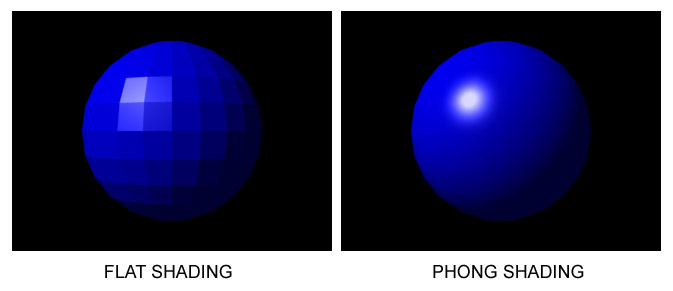
\includegraphics[width=\textwidth]{phong}
    \caption{Плоское освещение и освещение по Фонгу.}
\end{figure}

Для демонстрационных целей в работе был использован шейдер, взятый из блога Hextant Studios\cite{FlatShader}. Результирующий плагин будет независим от конкретного шейдера, и в нём будет реализована поддержка отдельных материалов для листьев и ствола.



\section{Генерация листьев}
Разработка была начата с генератора \emph{круглой листвы}. Для этого были изучены руководства по моделированию в стиле low poly, чтобы максимально приблизить программную реализацию генератора к тому, как моделирует человек.

Генерация листьев проходит в несколько шагов:
\begin{enumerate}
\item Генерируется модель икосаэдра радиусом в одну единицу. У икосаэдра 12 вершин с координатами 
(\texttt{\(0, \pm\Phi, \pm1\)}), 
(\texttt{\(\pm1, 0, \pm\Phi\)}), 
(\texttt{\(\pm\Phi, \pm1, 0\)}) и 20 треугольных граней.\cite{IcosahedronMath}
Векторы вершин нормализуются, чтобы привести радиус фигуры к единице. Также фигура поворачивается на случайный угол.

Для описания поворотов в трёхмерном пространстве в компьютерной графике широко применяются \emph{кватернионы}. Кватернион - это гиперкомплексное число, образующее векторное пространство размерностью четыре над полем вещественных чисел, которое можно представить как сумму вида

\begin{equation}
    q = a + bi + cj + dk,
\end{equation}

где $i$, $i$, $k$ - мнимые единицы, такие, что $i^2 = j^2 = k^2 = ijk = -1$. Свойства кватернионов делают их удобным инструментом для описания вращения\cite{quaternions}.

В Unity кватернионы представлены классом \texttt{Quaternion}. Для получения случайного поворота существует свойство \texttt{Random.rotation}. Кватернион умножается на вектор для поворота последнего, причём операция не ассоциативна и кватернион должен быть первым операндом, а вектор - вторым. Таким образом, чтобы повернуть модель, надо умножить кватернион на каждую её вершину.

\item Для увеличения количества граней применяется \emph{алгоритм подразделения}\cite{Subdivision}, который применяется для создания икосфер. Икосфера - это приближённый к сфере многогранник, полученный путём разделения каждой грани на четыре и последующего смещения новых вершин на поверхность описанной сферы. На рисунке ~\ref{fig:subdivision} показан пример икосферы, полученной с использованием двух итераций подразделения.
 
\begin{figure}[h]
    \centering
    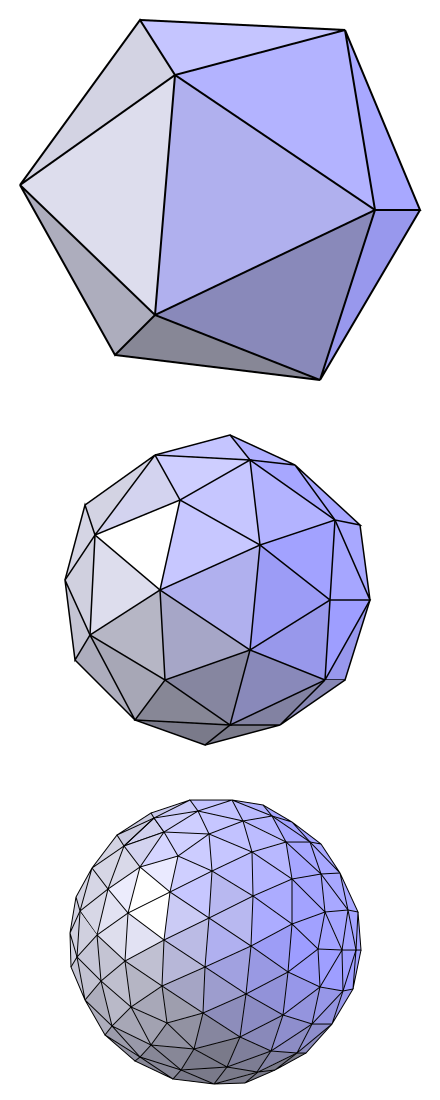
\includegraphics[height=0.5\textwidth, angle=90]{subdivision}
    \caption{Пример двукратного подразделения икосаэдра. Автор: Simon Fuhrmann, Wikimedia}
    \label{fig:subdivision}
\end{figure}

В нашем случае достаточно всего одной итерации подразделения, которая повысит число полигонов с 20 до 80. Поскольку уровень детализации определяется автоматически, было решено использовать подразделение только для листвы, ширина или высота которой не меньше значения по умолчанию (3 единицы).

Блок-схема алгоритма подразделения приведена на рисунке ~\ref{fig:subdivisionFlowchart}.

\begin{figure}[h]
    \centering
    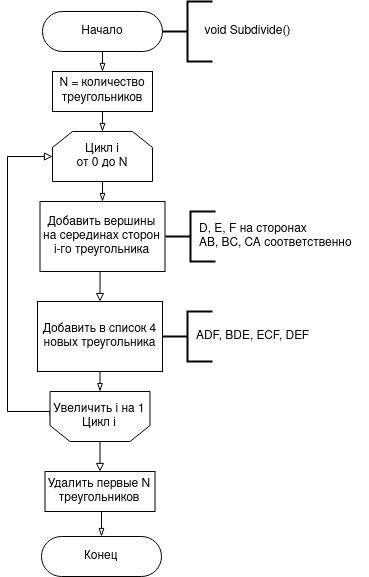
\includegraphics[width=0.6\textwidth]{subdivisionFlowchart}
    \caption{Блок-схема алгоритма подразделения.}
    \label{fig:subdivisionFlowchart}
\end{figure}

\item Фигура растягивается для достижения заданной ширины и высоты. Для каждой вершины вычисляется радиус (то есть длина вектора) по следующей формуле:

\begin{equation}
    r = lerp\left(width, height, \frac{\left|y_{v}\right|}{|v|}\right),
\end{equation}

где $lerp$ - функция линейной интерполяции, 

$width$ и $height$ - заданные ширина и высота листвы,

$v$ - вектор, задающий вершину.

\item Наконец, вершины случайным образом смещаются для придания листве более натурального вида. Однако если две вершины поменяются местами, то геометрия листвы будет нарушена, поскольку грани начнут пересекаться. Следовательно, для каждой вершины необходимо найти максимальный допустимый радиус смещения, при котором многогранник сохранит правильную форму.

Для нахождения максимального допустимого смещения используется следующая формула:

\begin{equation}
    maxshift_{i} = \frac{\displaystyle\min_{j = 0}^n(|V_{i} - N^{i}_{j}|)}{3}, 
\end{equation}
где $V$ - множество всех вершин, 

$N^{i}$ - множество соседей текущей вершины, 

$n$ - общее число соседей.

Полученное значение умножается на случайное значение от 0 до 1 и случайный единичный вектор, чтобы получить итоговое смещение для этой вершины.

Блок-схема алгоритма смещения вершин приведена на рисунке ~\ref{fig:displacementFlowchart}. 

\end{enumerate}

На рисунке ~\ref{fig:leaves} изображён пример листвы, сгенерированной с использованием вышеописанных алгоритмов.

\begin{figure}[h]
    \centering
    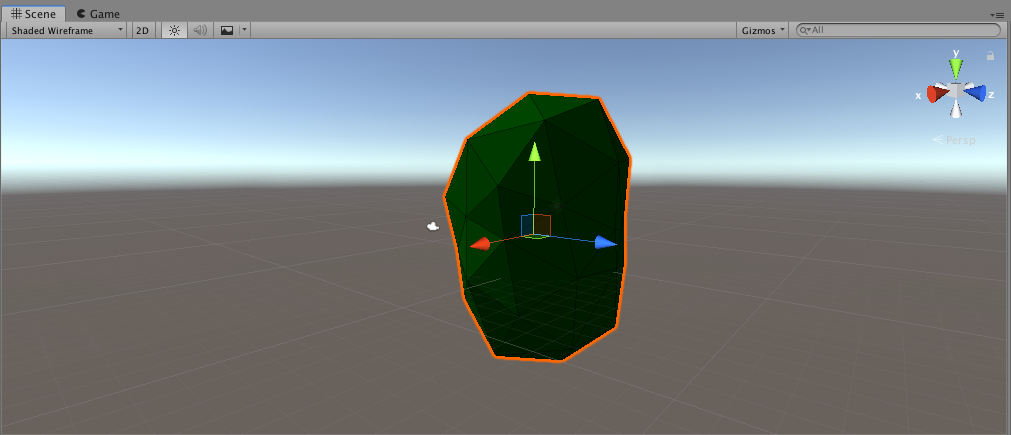
\includegraphics[width=0.8\textwidth]{leaves}
    \caption{Процедурно сгенерированная листва.}
    \label{fig:leaves}
\end{figure}



\begin{figure}[h]
    \centering
    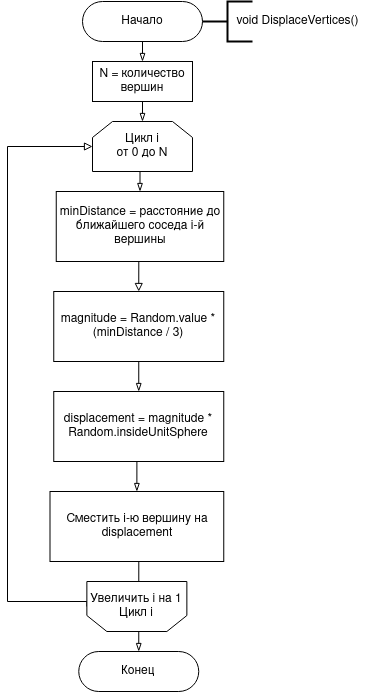
\includegraphics[width=0.5\textwidth]{displacementFlowchart}
    \caption{Блок-схема алгоритма смещения вершин.}
    \label{fig:displacementFlowchart}
\end{figure}

\section{Генерация ствола}
На первых этапах разработки генератора стволов был рассмотрен схожий проект\cite{hassank} на Github, посвящённый анимации роста процедурно генерируемых деревьев. Этот проект был заброшен на ранней стадии разработки, но алгоритм генерации ствола, используемый в нём, оказался полезен в данной работе; он был доработан и усовершенствован.

Ствол представляет собой пирамиду, разделённую на ярусы. Каждый ярус случайным образом поворачивается, задавая изгибы ствола. На конце ствола с помощью вышеописанного алгоритма генерируется крона, выделенная в отдельный игровой объект. Ствол состоит из 3-8 сегментов, количество которых пропорционально высоте.

На стволе также могут генерироваться ветви. С определённой вероятностью происходит выбор грани на текущем уровне, из которого может вырасти ветвь. Это возможно при условии, что высота текущего уровня не меньше 33\% от высоты дерева и не больше 90\%; это произвольно выбранные значения, предотвращающие генерацию ветвей в плохо подходящих для этого частях дерева. 

Второе условие генерации ветви заключается в том, что выбранная на уровне грань не должна быть направлена вниз, потому что ветвь не может расти вниз. Таким образом, нормаль выбранной грани должна иметь положительную компоненту по вертикальной оси. Также ветви не растут на деревьях с плоской листвой и хвоей.

Если эти условия выполнены, то создаётся объект генератора ветви и помещается в список, который будет обработан в последнюю очередь. Такое решение было принято для того, чтобы не нарушать порядок вершин, использованных в стволе. Ветвь начинает расти перпендикулярно стволу, но постепенно поворачивается вертикально вверх. 

Кроме того, с определённой вероятностью дерево может оказаться пнём. В таком случае оно будет обрублено в случайном месте. На срубе будет видна древесина и обломки коры. Пример такого пня представлен на рисунке ~\ref{fig:stumpResult}.

\begin{figure}[!htb]
    \centering
    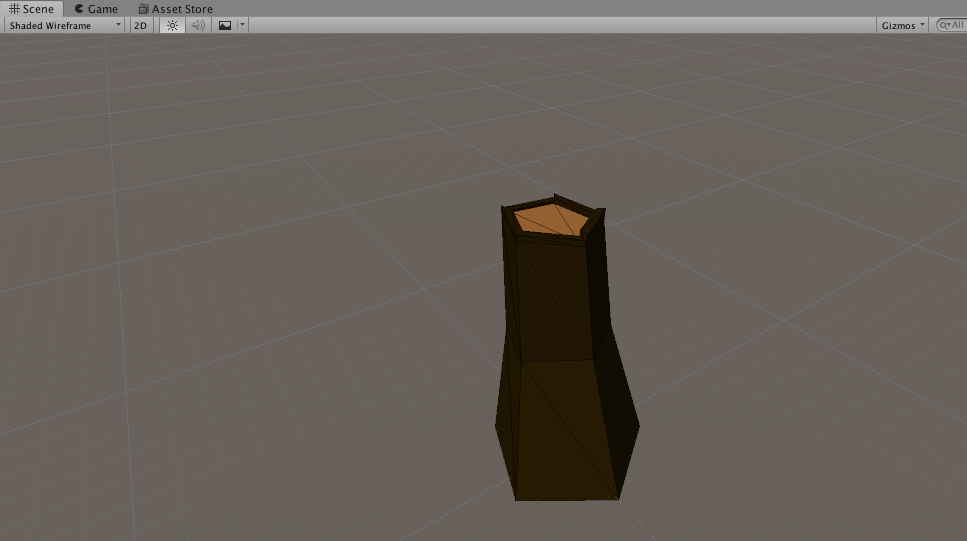
\includegraphics[width=0.8\textwidth]{stumpResult}
    \caption{Пример процедурно сгенерированного пня.}
    \label{fig:stumpResult}
\end{figure}

Блок-схема полного алгоритма генерации ствола приведена на рисунке ~\ref{fig:trunkFlowchart}.

На рисунке ~\ref{fig:roundResult} изображён пример процедурно сгенерированного дерева с круглой листвой.

\begin{figure}[!htb]
    \centering
    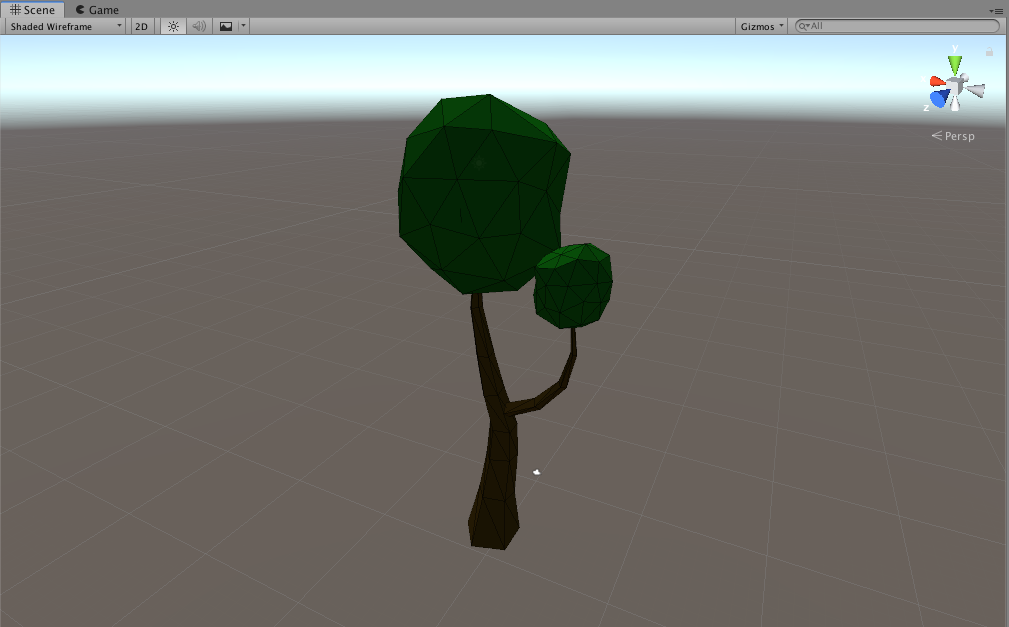
\includegraphics[width=0.8\textwidth]{roundResult}
    \caption{Пример процедурно сгенерированного дерева с круглой листвой.}
    \label{fig:roundResult}
\end{figure}

\begin{figure}[!htb]
    \centering
    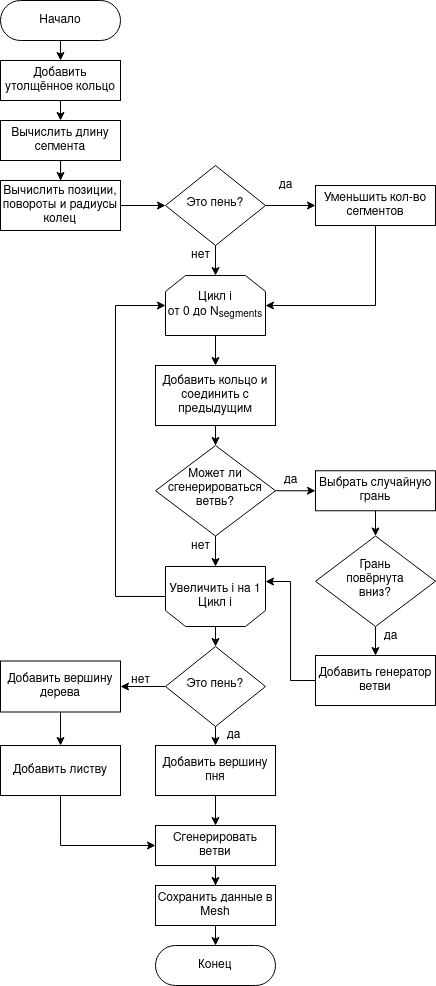
\includegraphics[width=0.6\textwidth]{trunkFlowchart}
    \caption{Блок-схема генерации ствола.}
    \label{fig:trunkFlowchart}
\end{figure}

\section{Генерация плоской листвы}
Разработанное расширение для редактора позволило ввести новые типы листьев, первым из которых стали \emph{плоские листья}, основанные на листьях пальм и древовидных папоротников. В реальности листья пальм имеют перистую либо веерную структуру, однако в силу минимализма графики в low poly для изображения пальмового листа обычно используют простую цепочку из полигонов. Иногда на её стороны добавляются ``насечки'', символизирующие перья. На рисунке ~\ref{fig:palmExample} изображена пальма в стиле low poly.

\begin{figure}[!htb]
    \centering
    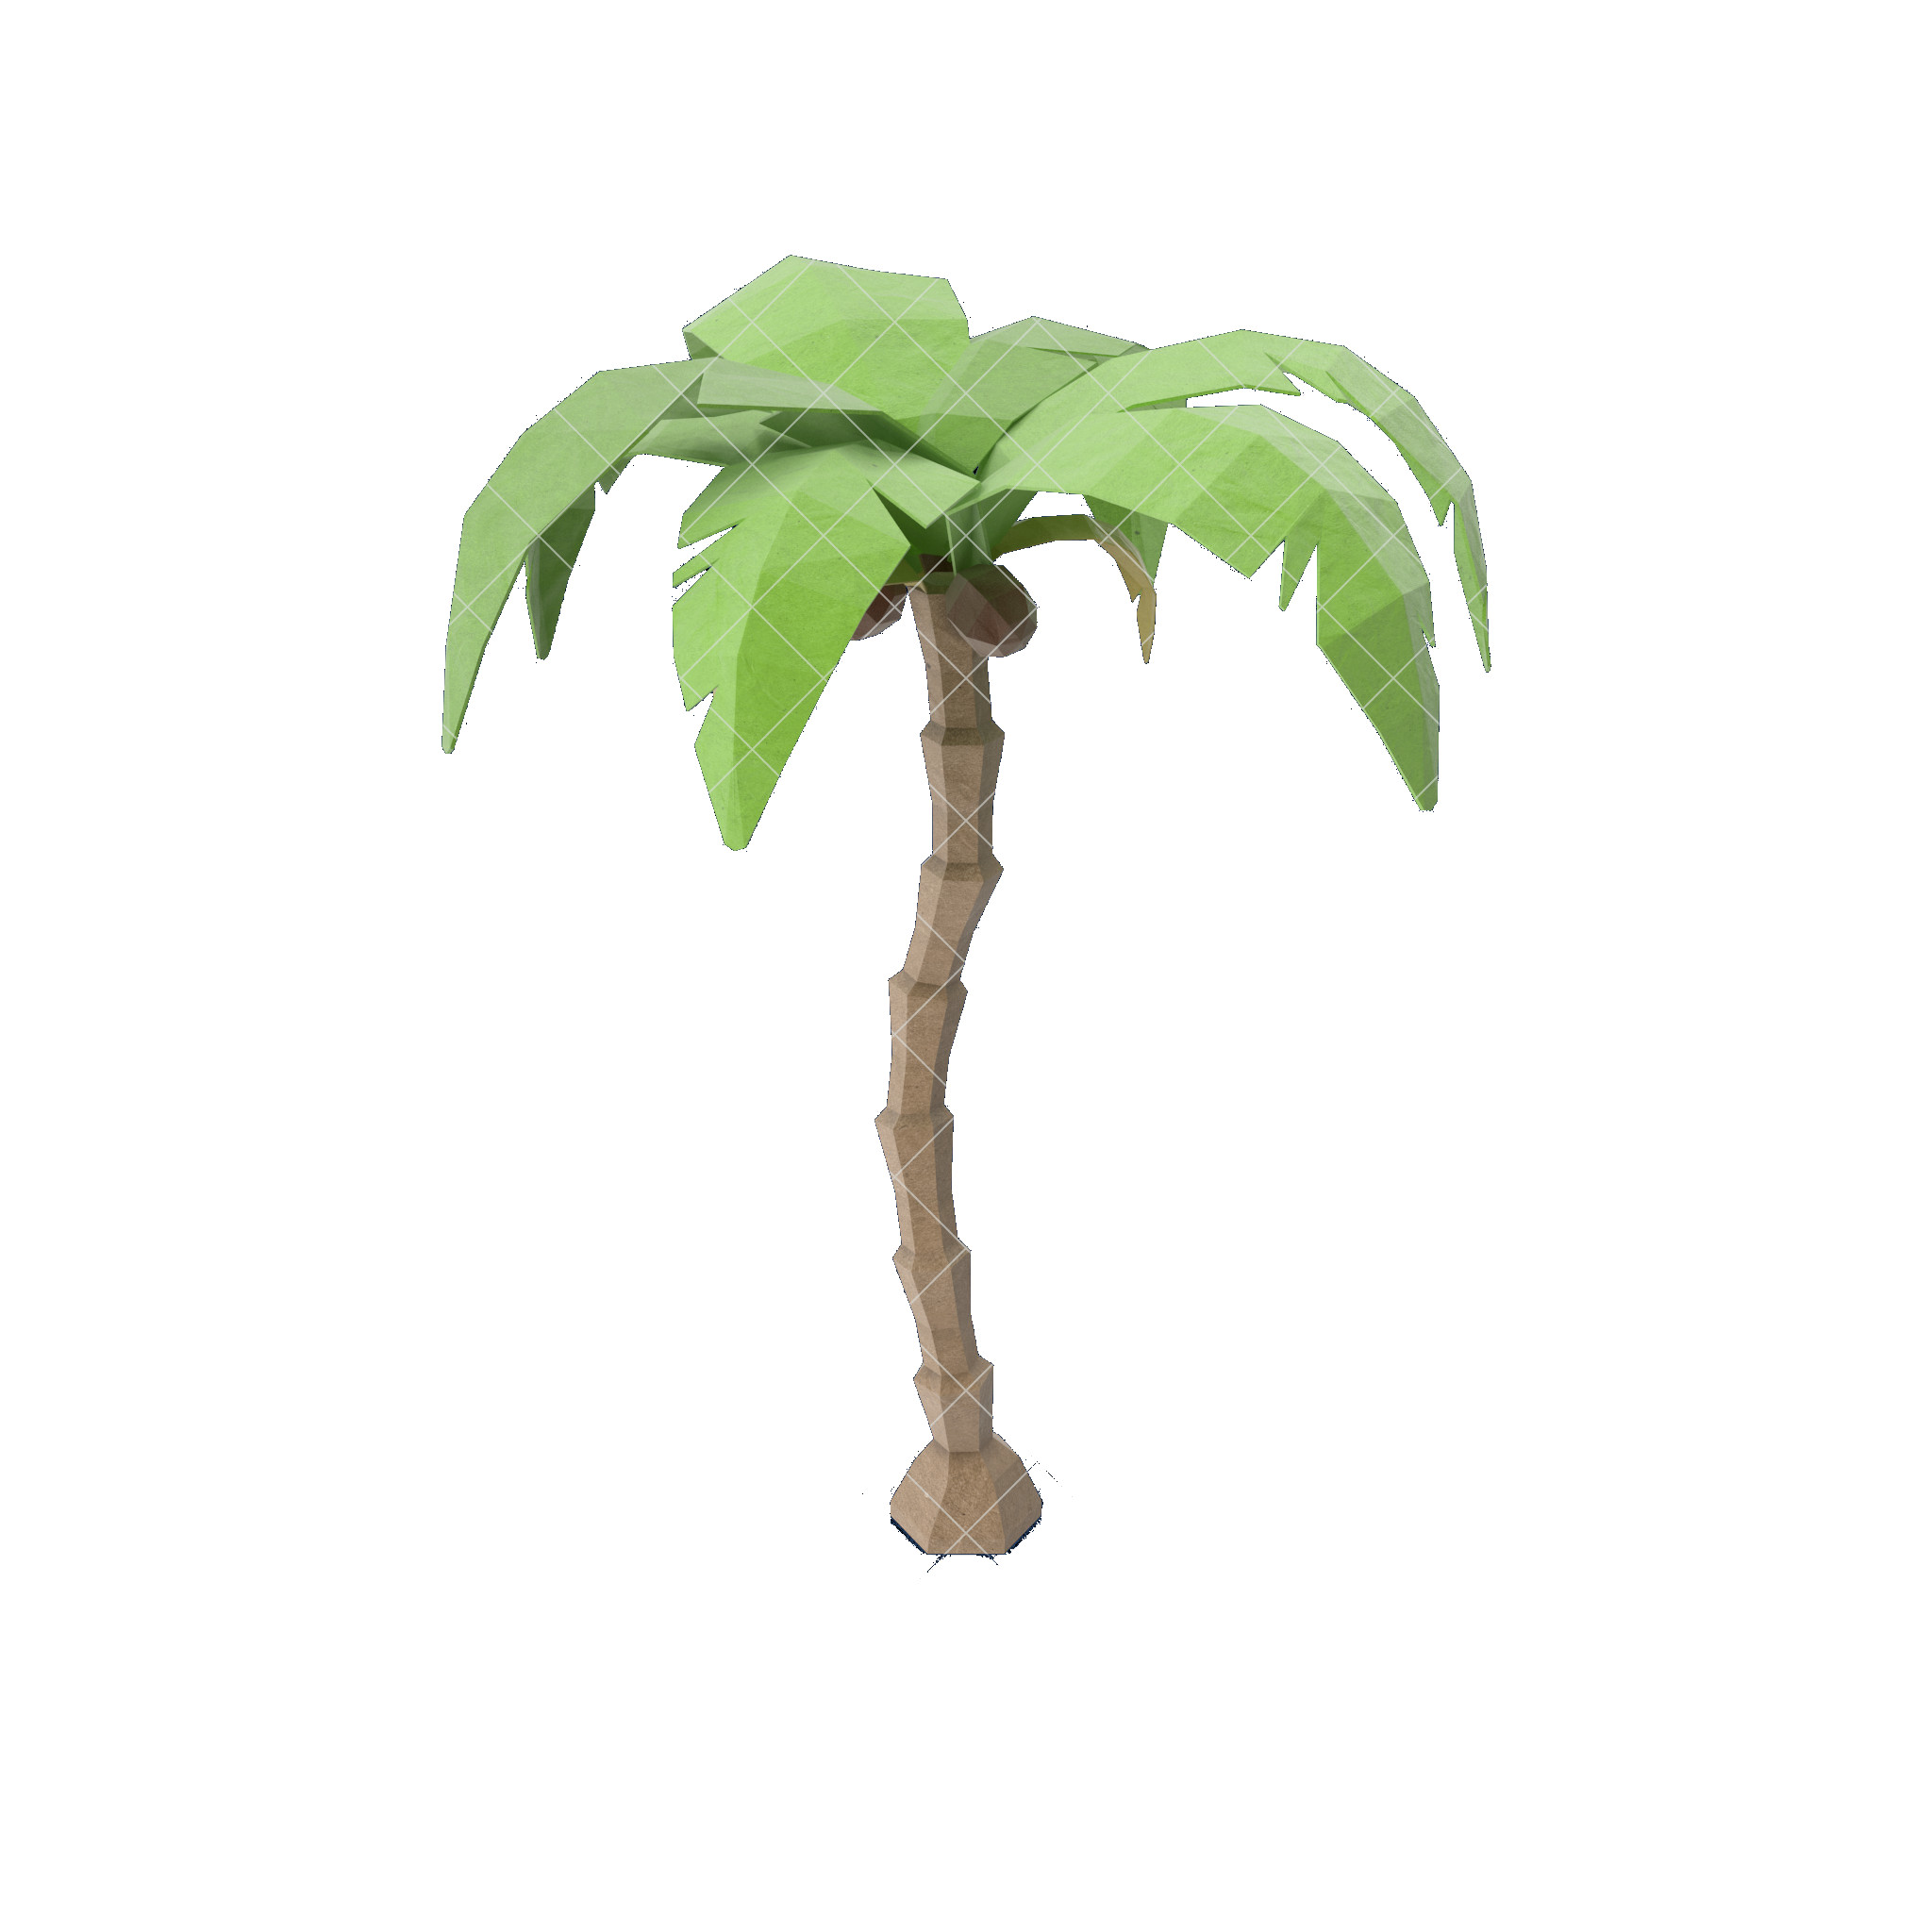
\includegraphics[width=0.6\textwidth]{palmExample}
    \caption{Пример пальмы в стиле low poly. Автор: bgaj23, pixelsquid.com}
    \label{fig:palmExample}
\end{figure}

Для описания формы листьев были использованы квадратичные кривые Безье.  Кривые Безье - это тип кривых, предложенный инженером из компании Renault Пьером Безье в 1962 году. Изначально эти кривые применялись для проектирования кузовов автомобилей, но впоследствии нашли широкое применение в компьютерной графике, где используются для рисования плавных изгибов. На рисунке ~\ref{fig:bezier} дано несколько примеров таких кривых. 

Кривые Безье обладают рядом свойств, благодаря которым они хорошо подходят для использования в компьютерной графике. Их основная ценность заключается в том, что они описываются опорными точками, при перемещении которых кривая изменяется интуитивно понятным образом. Однако кривая Безье не является интерполяцией; как видно по рисунку ~\ref{fig:bezier}, опорные точки не лежат на самой кривой, за исключением первой и последней. 

\begin{figure}[!htb]
    \centering
    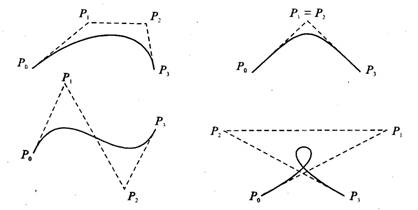
\includegraphics[width=0.6\textwidth]{bezier}
    \caption{Примеры кривых Безье.}
    \label{fig:bezier}
\end{figure}

Кривые Безье задаются рекурсивным выражением, благодаря чему они позволяют описывать сколь угодно сложные кривые. Тем не менее, в целях оптимизации вычислений на практике, как правило, применяются сочетания нескольких кривых небольших порядков. 

Теперь перейдём к формальному определению этого понятия. Кривая Безье порядка $n$ - это плоская полиномиальная кривая, которая задаётся следующим рекурсивным выражением\cite{BezierCurves}:
\begin{equation}
    B_{P_0}(t) = P_0
\end{equation}
\begin{equation*}
    B_{P_{0}...P_{n+1}}(t) = (1 - t) B_{P_{0}...P_{n}}(t) + tB_{P_{1}...P_{n+1}}(t),
\end{equation*}
где \(P_{0}...P_{n}\) - опорные точки. 

Как видно из этого выражения, у квадратичной кривой Безье три опорных точки: $P_0$, $P_1$ и $P_2$. Она имеет форму параболы и определяется следующим выражением:
\begin{equation}
    B(t) = (1 - t)^{2}P_{0} + 2t(1 - t)P_{1} + t^{2}P_{2}
\end{equation}

Таким образом, первая и последняя контрольные точки должны быть размещены в начале и конце листа соответственно, а центральная - посередине со смещением вверх, чтобы регулировать высоту. Это позволит создать лист параболической формы. 

Толщина листа достигает максимума в центре и линейно убывает по мере приближения к концам. Для её вычисления используется формула:
\begin{equation}
    segmentWidth = lerp\left(maxWidth, 0, 2\left|t - \frac{1}{2}\right|\right),
\end{equation}
где $maxWidth$ - заданная в редакторе ширина листа и $t$ - параметр интерполяции, равный 0 в начале листа и 1 в конце.

С заданным шансом на сегментах листа могут появляться треугольные вырезы, символизирующие перистую структуру. При этом сегмент будет состоять не из двух треугольников, как обычно, а из пяти, которые сходятся в одной общей вершине - конце выреза. Вырезы могут появляться на любой стороне сегмента листа или одновременно на обеих. Если на обеих сторонах сегмента появляется вырез, то этот сегмент разделяется надвое отрезком, соединяющим середины его внутренних сторон, и затем вышеописанная операция выполняется с каждой половиной. 

Пример процедурно сгенерированной пальмы показан на рисунке ~\ref{fig:flatResult}.

\begin{figure}[!htb]
    \centering
    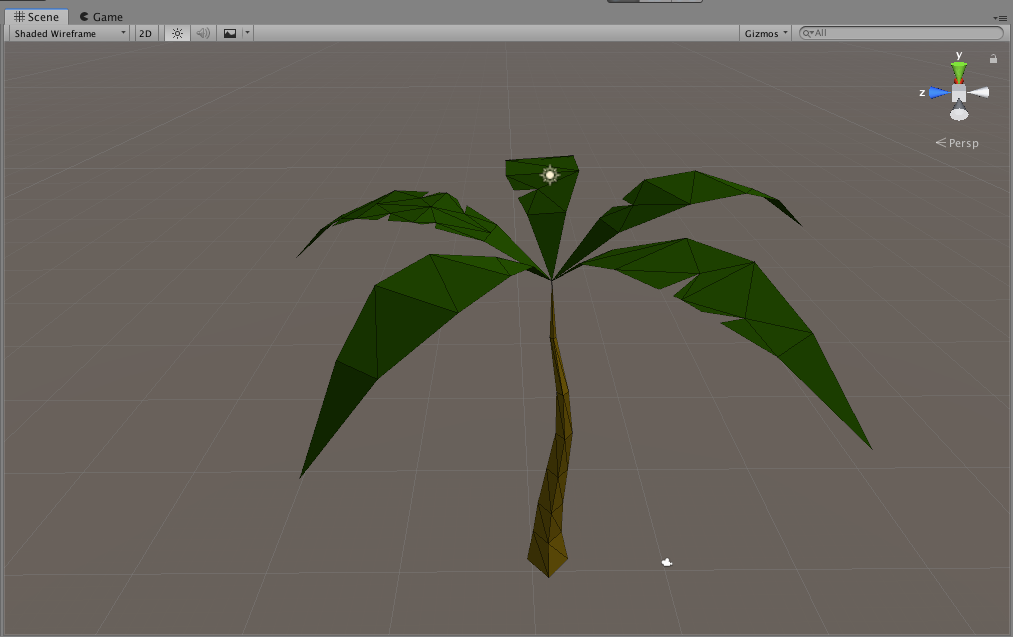
\includegraphics[width=0.6\textwidth]{flatResult}
    \caption{Пример процедурно сгенерированной пальмы.}
    \label{fig:flatResult}
\end{figure}

\section{Генерация хвои}
Последний тип листвы, реализованный в данном плагине - это хвоя. В low poly хвоя состоит из сложенных вертикально пирамид, облегающих ствол и повторяющих его изгибы. Для придания хвое более естественной формы каждую вторую вершину в основании яруса немного сдвигают вниз. На некоторых примерах с рисунка ~\ref{fig:pines} нижний ярус \'уже того, который находится над ним; эта деталь символизирует нижние ветви сосны, отмирающие из-за нехватки солнечного света.  

\begin{figure}[!htb]
    \centering
    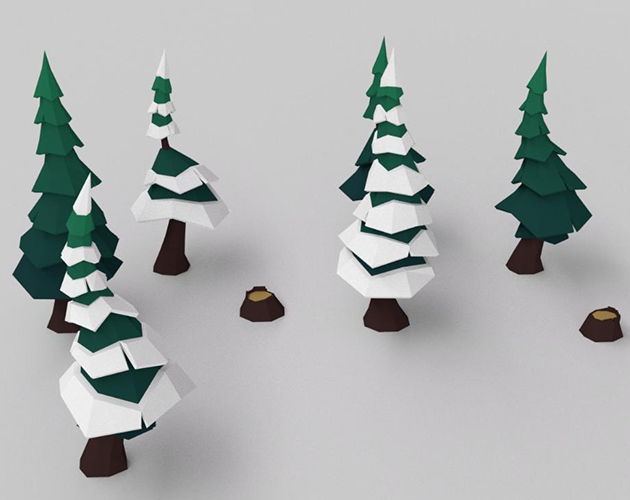
\includegraphics[width=\textwidth]{pines}
    \caption{Сосны в стиле low poly. Автор: TheTeaGuns, itch.io}
    \label{fig:pines}
\end{figure}

В отличие от других типов листвы, хвоя покрывает б\'ольшую часть ствола. По этой причине при генерации ствола необходимо сохранять позицию, поворот и радиус колец ствола, чтобы потом использовать их для генерации хвои. 

Процесс генерации хвои похож на генерацию ствола. Хвоя состоит из ярусов с чередующейся шириной, начинающих покрывать ствол после отступа в несколько сегментов снизу. Внешнее кольцо имеет радиус, равный сумме радиуса ствола и заданного радиуса листвы. Для внутреннего кольца к радиусу ствола прибавляется половина. 

Вначале определяется, будет ли нижний ярус узким. Если он узкий, то его радиус меньше обычного на половину радиуса листвы, а радиус внутреннего кольца яруса, следующего за ним - на четверть. Остальные ярусы генерируются по обычным правилам.

Вершины колец внешнего яруса, индексы которых имеют такую же чётность, что и индексы самого яруса, слегка сдвигаются вниз для придания хвое более естественной формы. Таким образом, на чётных ярусах сдвигаются чётные вершины, а на нечётных - нечётные. 

На рисунке ~\ref{fig:coniferResult} показан пример процедурно сгенерированного дерева с такой листвой. Деревья с хвоей не могут иметь ветви.

\begin{figure}[!htb]
    \centering
    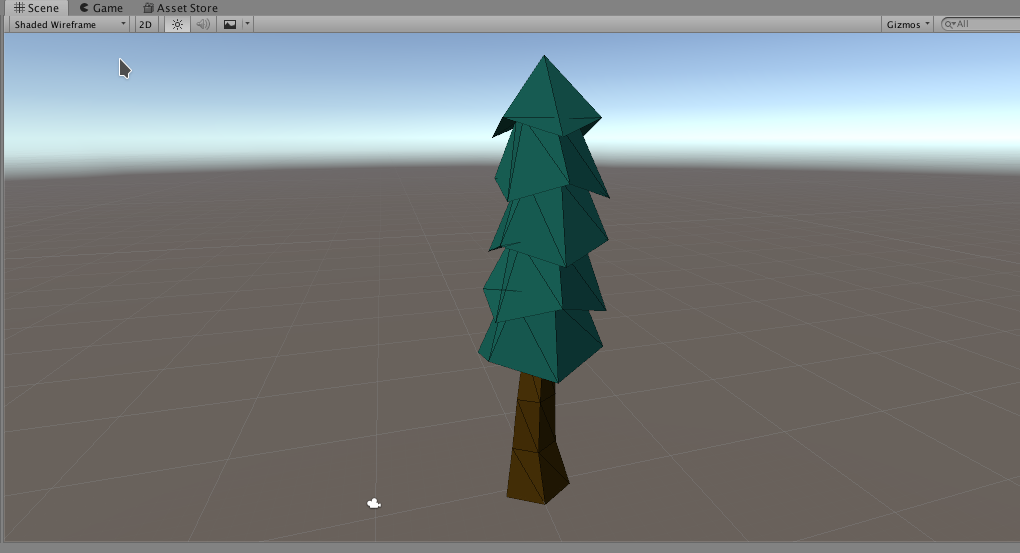
\includegraphics[width=0.8\textwidth]{coniferResult}
    \caption{Пример процедурно сгенерированного хвойного дерева.}
    \label{fig:coniferResult}
\end{figure}

\section{Разработка расширения для редактора}
В данном плагине была реализована возможность генерации различных типов листвы - круглой, плоской и хвои. Для удобной настройки генерации в редакторе должны отображаться только те параметры, которые относятся к выбранному типу листвы. Чтобы решить эту задачу, было создано расширение для редактора.

Стандартный редактор содержит компоненты интерфейса для задания значений общедоступных полей скрипта. Так, для строк используется поле ввода, для булевых значений - переключатель, для цветов - меню выбора цвета и так далее. Для чисел используется ползунок, если с помощью атрибута Range задан диапазон допустимых значений, а в противном случае - поле ввода. 

С помощью атрибутов можно добавить заголовки, изменить отображаемые в редакторе названия полей, скрывать поля из редактора, добавлять всплывающие подсказки и проводить некоторые другие манипуляции. Тем не менее, если этого недостаточно, Unity позволяет создать свой класс редактора для определённого скрипта.

Как и скрипты, расширения для редактора Unity пишутся на языке C\#. Класс расширения редактора должен наследоваться от класса Editor и находиться в одноимённой папке в корне проекта, чтобы Unity мог его зарегистрировать. Для того, чтобы привязать редактор к соответствующему объекту, используется атрибут CustomEditor\cite{UnityEditor}.

Создав своё расширение для редактора, разработчик может манипулировать свойствами редактируемого объекта в сериализованном виде. Сериализация скриптов в Unity нужна для обеспечения работы механизма горячей перезагрузки, благодаря которому редактор сохраняет значения параметров при изменении скрипта. 

Пользовательская логика отображения редактора должна находиться в методе \texttt{OnInspectorGUI}. Сериализованный объект хранится в поле \texttt{serializedObject}, а метод \texttt{FindProperty} позволяет получить доступ к его свойствам. Затем c помощью класса \texttt{EditorGUILayout} выводятся компоненты интерфейса, используемые для изменения значений полей. Наконец, после отрисовки интерфейса необходимо вызвать метод \texttt{serializedObject.ApplyModifiedProperties}, который запишет все изменения из объекта C\# в память.

\begin{figure}[!htb]
    \centering
    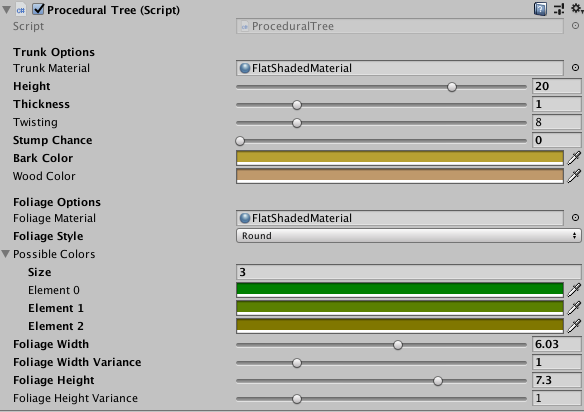
\includegraphics[width=0.8\textwidth]{editor}
    \caption{Интерфейс разработанного расширения редактора.}
\end{figure}

Разработанное расширение позволяет скрывать или отображать  параметры в зависимости от выбранного типа листвы, определяемого полем \texttt{Foliage Style}. Если выбран тип \texttt{None}, то все параметры скрываются, а листва не генерируется.

\newpage
